\documentclass{article}
\usepackage[utf8]{inputenc}

\title{Main Locations Extraction in Literature}
\author{Ohad Edelstein (ID 039065313), Nitzan Katz (ID 318446929)}
\date{Submitted as final project report for NLP, IDC, 2020}

\usepackage{natbib}
\usepackage{graphicx}
\usepackage{hyperref}
\usepackage{wrapfig}
\usepackage{xcolor,colortbl}

\begin{document}

\maketitle

\section{Introduction}

The purpose of this project is to extract the locations related to main characters in books. This may contribute to a bigger task of making a site-seeing route based on the route of main characters in archaeology books. The project includes POS (part of speech) tagging and NER (name entity recognition) in books, characters relational graph based on sentiment analysis and characters-locations co-occurrences graph. We mostly rely on commonly used models for solving this issue rather than inventing new models for the specific tasks.

\subsection{Related Works}
The main work we referred to is a github project\cite{hzjken2019char} in which the author extracted the characters out of the harry potter series, and made two types of relational graph between them. One graph is made based on co-occurrences of the characters in the books, and the other was made using sentiment analysis over the sentences more than one character was involved in order to determine the nature of the relationship (whether it's good or bad, and how strong it is). We thought about taking this concept and checking if the characters with the most relations to other characters can be classified as the main characters, and furthermore use the co-occurrences of those characters to locations to determine the main locations from the book.

\pagebreak
\section{Solution}
\subsection{General approach}
We started the project with a wide internet research on character detection in books. The initial idea was to find an approach for extracting the interesting characters in books and try to convert it to locations instead.\newline
Shortly into the reading we found the main project we relied on, with the general idea of making a relation graph between the characters in a book to find its main characters. We wanted to try and see if the same technique can be used to find the main locations of the book based on their connections with the main characters.\newline
The project focused only on the Harry Potter series, which is nice for a proof-of-concept for the characters idea, but since most of the names and locations are made up, we soon found out that locations identification isn't that straight forward. However, our main goal is archaeology books with real places, so we decided to keep going with the idea and try it on other books with stories happening in real locations (Patriot Games by Clancy Tom).

\subsection{Design}
The original project is made out of 5 parts in general: Data Preparation for the processing parts, NER for retrieving the characters and locations, character importance to filter out the non-interesting characters, co-occurrence matrix to find relations between characters and places and sentiment matrix to see the kind of relations.
\subsubsection{Data Preparation}
Before the processing of the data itself we need to prepare the data to work on. That involves both getting the novels, which we got from the project Gutenberg\cite{projectgutenberg}, and defining a list of commonly used words in English in order to filter out words from the NER process that got mis-tagged. We just used the same definition as the one used in the original project.
\subsubsection{Name Entity Recognition}
For the NER task we used the SpaCy NER classifiers\cite{spacy}, which are pre-trained classifiers that are commonly used in such projects (Both model used trained over the OntoNotes 5\cite{ontonotes} with one model using GloVe vectors). At this part, we go over each sentence from the book and extract the names and the locations. At this part, we also split the full names into the words, that's because sometimes a character is being referred by its full name, and sometimes by its first/last name instead. After that names that are in the common English words list are removed, and names that appear less than a certain threshold are removed (to filter outliers and very uncommon characters).
\subsubsection{Character Importance}
The character importance is determined mostly by the appearances of that character in the book. With the same concept, we filter the important places by the places that appeared the most in the book. With a smaller set of names and locations the calculation and visualization of the relations graphs becomes possible in relatively small amount of time.
\subsubsection{Co-occurrence Matrix}
The co-occurrence matrix is calculated solely on the appearance of two characters (and character and a location) in the same sentence, since this is the method in which we go over the book. The method is simple, we first create a binary indication for each sentence and word if the word appeared in the sentence, then we just multiply the matrix by itself to find the cross-appeared words. After that, we triangularize the matrix since it's symmetrical, and remove the diagonal values because we don't mind words that appear with themselves. The process is described in figure 1.
\begin{figure}[h]
  \centering
  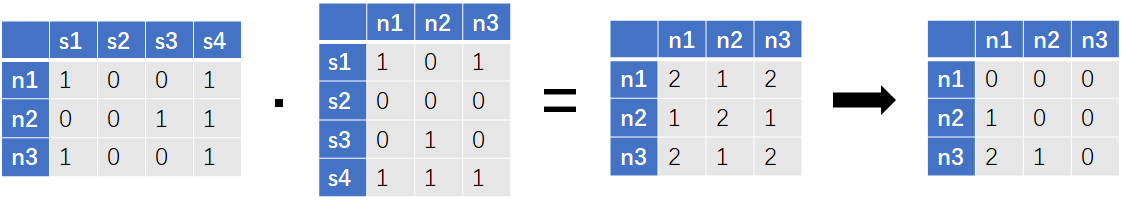
\includegraphics[width=10cm]{co-occurences_defintion.png}
  \caption{Co-occurrence Matrix Build}
  \label{fig1}
\end{figure}
After the matrix is created, we can easily turn it into a graph, normalizing the color of the edge of each connection by the amount of relations related to the others in the matrix.

\subsubsection{Sentiment Matrix}
The 

\section{Experimental results}

\section{Discussion}

\section{Code}


\bibliographystyle{plain}
\bibliography{references}

\end{document}